% !TEX root = ./main.tex
\section{Oligo Pool Design} \label{sec:oligo_pool}
\subsection{Identification of Transcription Start Sites}
All oligo pools used in this work were manually designed. For each gene in our list we looked for promoters in Ecocyc \cite{keseler2010ecocyc} (accessed 12/08/2021) using the transcription start site if the promoter was found. If multiple promoters were identified, each promoter was included in the experiment. If no promoter was found, we looked for transcriptionally active sites in the data set from Urtecho et al, 2020\cite{urtecho2020genome}. In their work, every part of the genome was tested for transcription initiation in LB. If we could find a site that was identified as active close to the gene of interest, we chose this site as origin for computational promoter mutagenisis. If no transcription start site could be identified for a gene, the model from \cite{la2021automated} was used to computationally predict a transcription start site in the intergenic region. The site predicted to be the most active within 500 bp upstream of the coding region was chosen as transcription start site since more than 99\% of transcription start sites are within that region in \textit{E. coli} K12 MG1655, see Fig.~\ref{fig:tss_distance}. Restriction enzymes leaving compatible sticky ends to the digested plasmid were used to cut the RiboJ::sfYFP element.  

\begin{figure}
    \centering
    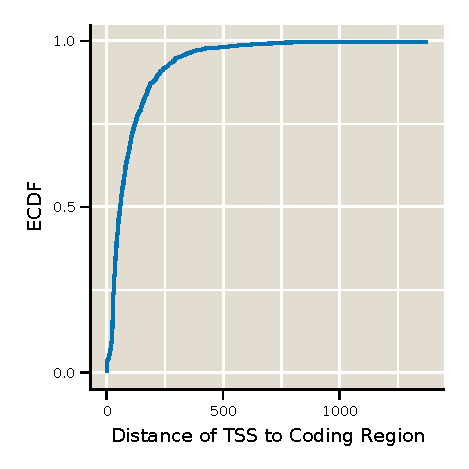
\includegraphics{../figures/tss_CR_distance.pdf}
    \caption{ECDF of distances of transcription start sites to the coding region for every operon in \textit{E. coli} that has a transcription start site annotated in EcoCyc. }
    \label{fig:tss_distance}
\end{figure}


\begin{figure}
    \centering
    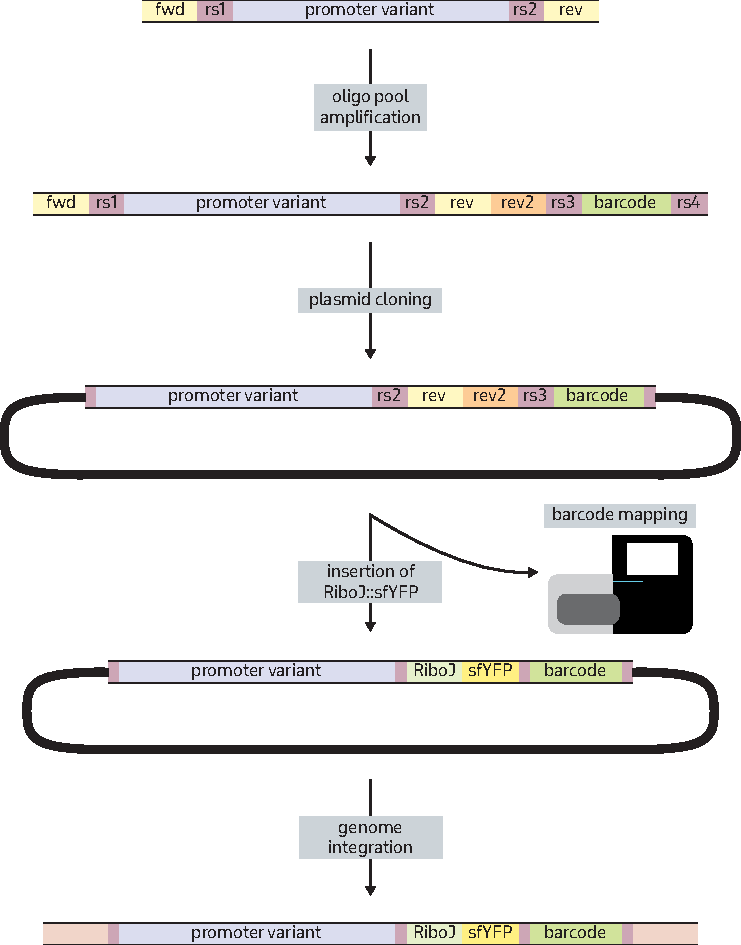
\includegraphics{../figures/cloning_scheme.pdf}
    \caption{Placeholder figure for cloning scheme.}
    \label{fig:cloning}
\end{figure}

\subsection{Computational Promoter Mutagenesis}
Once a TSS is identified, the 160 bp region from 115 bp upstream of the TSS to 45 bp downstream is taken from the genome. It has been shown that most cis-regulation is happening within this window \cite{rydenfelt2014statistical}. Based on the approach by \cite{kinney2010using}, each promoter sequence is mutated randomly at a rate of 0.1 per position. 1500 mutated sequences are created per promoter, following the approach from \cite{ireland2020deciphering}, which creates sufficient mutational coverage across the window. The promoter oligonucleotides are flanked by restriction enzyme sites (\textit{rs1} and \textit{rs2} in Fig.~\ref{fig:cloning}) that are used in downstream cloning steps. The restriction sites are flanked by primer sites used to amplify the oligo pool. Primer sequences were chosen from a list of orthogonal primer pairs, designed to be optimal for cloning procedures \cite{subramanian2018set}. oligo pools were synthesized (TwistBioscience, San Francisco, CA, USA) and used for subsequent cloning steps.


\section{Library Cloning}
\subsection{Cloning oligo pool into plasmid vector}
\label{sec:library_cloning}
The oligo pool was amplified using a 20bp forward primer (SC142) and a 40 bp reverse primer (SC143), which consists of 20bp primer binding site and 20bp overhang. PCR amplifications were run to minimal amplification to minimize amplification bias. PCR products were cleaned and concentrated (DNA Clean \& Concentrator-5, ZymoResearch) and used for a second amplification step. The 20 bp overhang from the first amplification was used as primer site for a reverse primer (SC172), which contains randomized 20 bp barcode, flanked by two restriction enzyme sites (\textit{rs3} and \textit{rs4} in Fig.~\ref{fig:cloning}). The forward primer is the same as in the first amplification step. PCR amplification is run again to minimal amplification to minimize amplification bias. PCR products are run on a 2\% agarose TAE gel and subsequently extracted and purified (Zymoclean Gel DNA Recovery Kit, ZymoResearch). In the next step, restriction digest is performed on the outer restriction enzyme sites (\textit{rs1} and \textit{rs4} in Fig.~\ref{fig:cloning}). Unless noted otherwise, all restriction digests were run for 15 minutes at 37C. The plasmid vector was digested with different restriction enzymes which create compatible sticky ends. Most restriction enzyme sites are palindromes, so by choosing different enzymes with compatible ends, we avoid having palindromes flanking the plasmid inserts. This is important, since these sites are used for amplifications in the library preparation steps later in the protocol. (\purple{Maybe not needed to say}). The oligo pool is combined with the plasmid vector using T7 DNA ligase (New England Biolabs, Ipswich, MA, USA) following the suppliers protocol. Ligation products were cleaned and concentrated (DNA Clean \& Concentrator-5, ZymoResearch) and drop dialysis (MF-Millipore VSWP02500, MilliporeSigma, Burlington, MA, USA)  was performed for 1h to improve sample purity. Electroporation using \textit{E. coli} pir116 electrocompetent cells (Lucigen, Middleton, WI) was performed at 1.8kV in 1mm electroporation cuvettes, followed by 1h recovery at 37C and 250rpm in 1 ml LB-media (\purple{details here}, the same for all following mentionings of LB). The entire cultures were plated on 150mm kanamycin (50$\mu$g/ml) + LB petri dishes and grown overnight. The following day, plates were scraped and the colonies resuspended. Freezer stocks were prepared using a 1:1 dilution of resuspended colonies and 50\% glycerol. Cultures were inoculated with $5\times 10^8$ cells in 200ml of LB + kanamycin (50$\mu$g/ml) and grown at 37C until saturation. Plasmid was extracted (ZymoPURE II Plasmid Maxiprep Kit, ZymoResearch) and used subsequent sequencing (see \ref{sec:barcode_mapping}). The plasmid library is then used as template in a restriction digest using restriction enzymes $rs2$ and $rs3$. The resulting product was cleaned and concentrated (NEB Monarch) and concentration measured on a Nanodrop. Similarly, the riboJ::YFP element was PCR amplified (primers SC191 and SC192), adding restriction sites as overhangs (see table \ref{tab:re_sites}). The PCR product was cleaned and concentrated (NEB Monarch) and digested with the respective restriction enzymes. The plasmid library is combined with the RiboJ::sfYFP element using 7 DNA ligase (New England Biolabs, Ipswich, MA, USA) following the suppliers protocol. Ligation products were cleaned and concentrated (NEB Monarch) and drop dialysis (MF-Millipore VSWP02500, MilliporeSigma, Burlington, MA, USA)  was performed for 1h to improve sample purity. Electroporation using \textit{E. coli} pir116 electrocompetent cells (Lucigen, Middleton, WI) was performed at 1.8kV in 1mm electroporation cuvettes, followed by 1h recovery at 37C and 250rpm in 1 ml LB-media. The entire cultures were plated on 150mm kanamycin (50$\mu$g/ml) + LB petri dishes and grown overnight. The following day, plates were scraped and the colonies resuspended. Freezer stocks were prepared using a 1:1 dilution of resuspended colonies and 50\% glycerol. Cultures were inoculated with $5\times 10^8$ cells in 200ml of LB + kanamycin (50$\mu$g/ml) and grown at 37C until saturation. Plasmid was extracted (ZymoPURE II Plasmid Maxiprep Kit, ZymoResearch) and used for subsequent genome integration. 


\section{Barcode Mapping}
\label{sec:barcode_mapping}
The plasmid library is used for barcode mapping. Purified plasmid is PCR amplified using forward primer (SC185) outside the promoter region and a reverse primer outside the 20bp barcode (SC184). The PCR is run to minimal amplification (until a band is visible on an ararose gel), and the product is gel purified (NEB Monarch). The purified DNA was used as template for a second PCR using a primer (SC196) adding an Illumina P5 adapter to the promoter side, and a primer (SC199) adding an Illumina P7 adapter. The PCR is again run to minimal amplification and gel purified (NEB Monarch). The product was used for sequencing on a Illumina NextSeq P2 flow cell with pair end reads using primers SC185 for read 1, SC184 for read 2 and SC201 for the index read. Reads were filtered and merged using custom bash scripts, which are available in the Github repository. After processing, each promoter/barcode pair was identified in each read, and pairs with less than 3 total reads were discarded. An alignment algorithm was used to identify the identity of each sequenced promoter variant. This allowed to include additional promoter variants that were in the initial oligo pool due to synthesis errors in the production of the oligos. The barcode mapping was used in analysis of libraries grown in various growth conditions.

\begin{table}[]
\centering
\begin{tabular}{|l|l|l|}
\hline
Part             & 5' restriction site & 3' restriction site \\ \hline
Plasmid Vector   & XbaI                & XhoI                \\ \hline
RiboJ::YFP       & ApaI                & PtsI                \\ \hline
Oligo Pool       & SpeI                & ApaI                \\ \hline
Barcoding Primer & SbfI                & SalI                \\ \hline
\end{tabular}
\caption{Restriction sites used. All enzymes were ordered from NEB (\purple{check which ones are high fidelity versions})}
\label{tab:re_sites}
\end{table}

\subsection{Genome Integration}
We used ORBIT to integrate the reporter libraries into the chromosome. A detailed description of the method and its efficiencies can be found in (\purple{Add scotts paper here}). Wild type \textit{E. coli} (K12 MG1655) are streaked on a LB plate and grown overnight at 37C. A single colony is picked and grown in 3ml of LB at 37C and shaken at 250rpm overnight. The overnight culture is diluted 1:1000 into fresh LB (e.g. 200ml) and grown at 37C and 250rpm until exponential phase ($\sim$ 0.4 OD 600nm). The cultures are then immediately put on ice and spun in a centrifuge at 5000g for 10min. Following the spin, the supernatant is discarded, and the cells are resuspended in deionized water at 4C at the same volume as the initial culture. The cells are spun again at 5000g for 10 min. This wash step is repeated 4 times with 10\% glycerol. After the last wash, supernatant is discarded and cells are resuspended in the remaining liquid and distributed into 50$\mu$l aliquots. Aliquots are frozen on dry ice and kept at -80C until used for electroporation. For electroporation, aliquots are thawed on ice and 1mm electroporation cuvettes are pre-chilled on ice. 100ng of helper plasmid (\purple{link to helper plasmid file}) is added to a 50$\mu$l cell aliquot and mixed by slowly pipetting up and down. The aliquot is then added to the electroporation cuvette and electroporation is performed at 1.8kV. The aliquot is recovered with 1ml of LB media prewarmed to 37C for an 1h prior to electroporation. The culture is recovered for 1h at 37C and shaken at 250rpm. After recovery, aliquots at various dilutions are plated on LB + gentamycin (\purple{check gent concentration}). Plates are grown overnight and a single colony is picked to prepare frozen stocks as described above. To perform genome integration, the host strain carrying the helper plasmid is made electrocompetent (follow growing and washing steps described above), and the plasmid library is electroporated into the host strain. The cells are recovered in 3ml of prewarmed LB + 1\% arabinosea and shaken at 37C at 250rpm for 1h. The entire volume is plated on LB + kanamycin plates \tr{add concentration} and colonies are grown over night. The next day, colonies are scraped, resuspended in LB and diluted to optical density of 1 at 600nm. The helper plasmid used for genome integration causes growth deficits, hence, the library needs to get cured of the plasmid. Therefore, the library is inoculated with 0.5ml of culture at 1 OD in 200ml of LB, and grown until exponential phase at 37C shaken at 250 rpm. The helper plasmid carries the \textit{sacB} gene, which is used for negative selection in the presence of sucrose. At exponential phase, the culture is plated on LB + 7.5\% sucrose agarose plates. Plates are grown overnight, scraped and made into frozen stocks. The frozen stocks are then ready for growth experiments.


\section{Growth Conditions and Culture Growth}
\label{sec:culture_growth}


\subsection{gDNA and RNA extractions}
\label{sec:dna_rna_extract}


\section{Barcode Sequencing}
\label{sec:barcode_seq}

\section{Supplementary Files}
\label{sec:SI_files}
\begin{itemize}
    \item Plasmid Sequences with annotations + RiboJ::YFP
    \item pHelper sequence
    \item Primers
    \item list of restriction sites used in cloning
    \item Gene list
    \item Sequencing Data
    \item List of ordered sequences
\end{itemize}